% Template for ESA-EUSC-JRC 2012 paper; to be used with:
%          spconf.sty  - LaTeX style file, and
%          IEEEbib.bst - IEEE bibliography style file.
% --------------------------------------------------------------------------
\documentclass{article}
\usepackage{spconf,amsmath,epsfig}
\usepackage{graphicx}
%\usepackage{relsize}

%\DeclareMathSizes{15}{15}{15}{15}


% Example definitions.
% --------------------
\def\x{{\mathbf x}}
\def\L{{\cal L}}

% Title.
% ------
\title{Artificial Generation of Big Data For Improving Image Classification: A Generative Adversarial Network Approach on SAR Data}

%
% Single address.
% ---------------
\name{*Dimitrios Marmanis\textsuperscript{1,3}, 
	  *Wei Yao\textsuperscript{1},
	  Fathalrahman Adam\textsuperscript{1},
	  Mihai Datcu\textsuperscript{1}, \\
	  \textit{Peter Reinartz}\textsuperscript{1},
	   \textit{Konrad Schindler}\textsuperscript{2},
  	   \textit{Jan Dirk Wegner}\textsuperscript{2},
	   \textit{Uwe Stilla}\textsuperscript{3}, \thanks{*Authors have contributed equally in this work}}

\address{\textsuperscript{1}Department of Photogrammetry  \& Image Analysis, German Aerospace Center (DLR), Germany \\
		\textsuperscript{2}Department Photogrammetry \& Remote Sensing, ETH Zurich,  Switzerland \\
		\textsuperscript{3}Department Photogrammetry \& Remote Sensing, Technische Universitaet Muenchen (TUM), Germany}
%
% For example:
% ------------
%\address{School\\
%	Department\\
%	Address}
%
% Two addresses (uncomment and modify for two-address case).
% ----------------------------------------------------------
%\twoauthors
%   { Dimitrios Marmanis*, \\ 
%   	 Wei Yao*, \\
%   	 Fathalrahman Adam*, \\
%   	 Mihai Datcu,\\
%   	 Peter Reinartz
%   	 \thanks{*Authors have contributed equally in this work}
%   	 }
%   { Department of Photogrammetry  \& Image Analysis, \\ 
%     Remote Sensing Technology Institute, \\ 
%   	 German Aerospace Center (DLR), Germany}
%   	 %
%   	 {K. Schindler, \\
%  	 J. D. Wegner }
%	 %  	 
%  	 {Photogrammetry \& Remote Sensing, \\
%  	 ETH Zurich, \\
%  	 Switzerland}
%   	 %   
%   {Dimitrios Marmanis, \\
%    Uwe Stilla }
%    %   
%   {Photogrammetry \& Remote Sensing, \\
%    Technische Universitaet Muenchen (TUM), \\
%    Germany}
   
\begin{document}
%\ninept
	\maketitle
%
\begin{abstract}

Very High Spatial Resolution (VHSR) large-scale \emph{SAR} 
image databases are still an unresolved issue 
in the Remote Sensing field.
In this work, we propose such a dataset for 
exploring patch-based classification from 
urban and peri-urban areas, considering $7$ 
distinct semantic classes.
In this context, we investigate the accuracy of 
large CNN classification models and pre-trained 
networks for SAR imaging systems. 
Furthermore, we propose a 
Generative Adversarial Network (GAN) for SAR image
generation and access if the derived data can 
actually improve classification accuracy, with no 
additional annotation.

\end{abstract}
%

% ============= KEYEOWRDS =========== %
\begin{keywords}
Big Data, SAR classification, GANs, Generative Adversarial Networks, Deep Learning
\end{keywords}
%

\section{Introduction}
\label{sec:intro}

Classification of very high resolution (VHR) \emph{SAR} 
image data remains still a hard and time-consuming task.
%
Some of the major difficulties involve, the scarcity 
of available data, the challenging interpretation of 
the semantic content and the particular characteristics
of the \emph{SAR} derived scattered signal.
%
All these important factors lead to a general absence of large
scale \emph{SAR-derived} image databases for Remote Sensing
image analysis and knowledge discovery.
%
Furthermore, despite the major advances on Big Data 
image classification, namely \emph{Deep Learning} methods, 
SAR-based systems have shown to benefit little from these 
important breakthroughs, mainly due to the limited 
availability of data and/or respective labels.

In this work we tackle the problem of limited
data by introducing and experimenting with a large-scale 
\emph{SAR} derived image database.
%
Precisely, our dataset contains more than $60000$ image 
instances and respective labels, chosen from $7$ distinct 
semantic classes.
%
Using this large-scale dataset, we perform a set of 
experiments for understanding the impact of 
data size in relation to classification accuracy. 
%
In this context, we also investigate the possibility of 
enhancing our dataset by generating artificial SAR images 
through the use of \emph{Generative Adversarial Networks} (\emph{GANs}).
Through this experiment, we access the possibility of artificial 
data generation for decreasing or completely avoiding the time-consuming 
data annotation process.
%
Our main contributions in this work can be summarized as follow:

\begin{itemize}  
  
  \item[$\bullet$] We construct the first large-scale pre-trained SAR image
  model, based on deep-learning Convolutional Neural Networks learning paradigm.

  \item[$\bullet$] We investigate the possibility of transfer-learning from other
  pre-trained computer-vision based models and their impact on SAR image classification.
  
  \item[$\bullet$] We investigate the impact of artificially derived SAR data over the 
  classification accuracy, by employing state-of-the art Generative Adversarial Networks (GANs).
  

\end{itemize}


\section{Related Work}
\label{sec:previous work}

In the field of SAR image analysis the use of deep-learning
methods, such as \emph{CNNs} models is still in its infancy stage, 
mainly due to limitations on availability of VHR data and 
respective labels.
%
Importantly, despite our detailed investigation in 
literature  we did not find any 
work employing large scale SAR-databases for 
alleviating the full potential of \emph{CNN-based} methods.
%
Furthermore, there are no available pre-trained, SAR-based 
models for facilitating the classification of small-size 
SAR image datasets.
    
Published work in the intersection of \emph{SAR} imaging
and deep-learning are mainly focusing on the topic of \emph{Target 
Classification}. Some representative works employ sparsely connected layers 
\cite{chen2016target}, limited training data 
\cite{lin2017deep} and domain-specific data augmentation 
methods \cite{ding2016convolutional}.
%
% For an overview of respective literature in the subject one can refer 
% to \cite{schwegmann2017development}.   
%
%Other interesting applications in the field include a CNN-based
%correspondence algorithm between SAR and optical-imagery 
%\cite{mou2017cnn} and SAR CNN-based despeckling algorithms 
%\cite{chierchia2017sar}.
In the field of \emph{GAN} model and \emph{SAR} data some interesting 
results have been proposed by \cite{guo2017synthetic}, where
authors constructed a generative framework.
%
The outcome of their experiments however had limited success due to the
scarce training data and particular characteristics of the underlying 
targets (military imagery). 
%
Another implementation of \emph{GANs} in the field 
of Remote Sensing is this of \cite{perezsemi}, where authors investigate the 
\emph{Wasserstein GAN} for poverty mapping with sparse labels using a 
semi-supervised approach. In this work however despite the interesting 
findings, results are not based on SAR imagery.
%
Yet another work on optical remote sensing imagery and artificial data 
generation is this of \cite{lin2016deep}. In this work the author proposes
an additional objective function over the standard GAN architecture, 
for improving the generated data. Despite the interesting framework however, 
the derived images are of poor quality and do not resemble any true semantic class.
%
A promising work is this of \cite{merkle2017possibility} where authors 
show high-quality image results on SAR generated images using as a 
base optical data.
%
The samples generated here are of exceptional quality, 
showing the potential of \emph{cGAN} 
methods in SAR image generation.

\section{The Dataset}
\label{sec:dataset}

Our dataset was obtained via a novel 
classification scheme especially designed
for high-resolution radar SAR imagery,  
mainly depicting built-up areas. 
%
The dataset contain information from $288$ 
TerraSAR-X image scenes ($41$ 
scenes are acquired from Africa, $6$ from 
Antarctica, $59$ from Asia, $80$ from Europe, 
$40$ from the Middle East, $54$ from North 
and South America and $8$ from ocean 
surfaces), with over $60000$ 
individual image patches.
%
All \emph{TerraSAR-X} data are obtained via
the X-band instrument using the high-resolution
Spotlight mode. The incident angle throughout the 
scenes varies between 20 and 50 degrees. The resolution
of the images scenes is set to $2.9$m with a pixel 
spacing of $1.25$m. 
The chosen polarization for the dataset
is set to horizontal model (HH) for all products.
Furthermore as a standarization process, we converted all
intensity data to 8-bit integer precision. 
% 
For more information on the dataset one can refer to
\cite{dumitru2016land}.

\section{Experiments}
\label{sec:experimnts}

In our experiments, we initially set a strong baseline 
through a deep-learning classification scheme and 
further investigate if we can improve accuracy
by introducing artificially \emph{GAN} generated data.

\subsection{The CNN SAR classifier}

As a baseline for our experiments, we
employ a state-of-the-art CNN classification architecture,
namely the Residual-Network that contains 50 hidden layers 
(\emph{ResNet-50}) \cite{he2016deep}. 
%
For our purposes, we remove the fully connected part of
the architecture and replace these layers with
three fully connected layers of size $256, 256$ and $7$ respectively. 
With this particular model, we achieve
an overall classification accuracy of $93.2\%$, 
proving the strong properties of CNN networks. 

\bigskip

\noindent
Yet another interesting observation is related with the fact that pre-trained
networks (optimum weights initialization) does not seem 
to affect the overall result. 
%
This may be a logical outcome, considering that pre-trained
networks are generally trained on standard RGB images that
bear very different properties with respect to \emph{SAR} images.
%
Under this observation, would be therefore normal to assume
that pre-trained weights do not to have any significant effect over the 
training process.
%
For proving this hypothesis, we trained our CNN network both
with random initialization weights and \emph{ImageNet} pre-trained weights.
The results in both case were similar with little to no-variation.

\subsection{Image Generation with BEGAN Models}
%
In this section, we investigate if artificial data generation through \emph{GAN}
models can actually improve our classification baseline.
%
Theoretically, such a task should be feasible considering previous
success is literature in tasks such as sign recognition \cite{wang2017adversarial}.
%
Our task however is much more challenging, considering the extreme variance of our
SAR dataset and the larger image dimensions required to be generated ($160 \times 160$ pixels).
%

\subsubsection{BEGAN Model Selection}

In the context of adversarial networks (\emph{GANs}), there is a plethora of model variations such 
as \emph{DC-GANs}, \emph{cGANs}, \emph{WGANs}, \emph{DRAGANs} and \emph{BEGANs}.
%
For our model, we decided to investigate the newly proposed \emph{BEGAN} model 
\cite{berthelot2017began}, as it has shown remarkable quality of generated image 
results, in addition to large image sizes.
%
%Precisely, even though other GAN variations fail to generate images
%larger than $64 \times 64$ pixels, \emph{BEGAN} can easily scale up to 
%$120 \times 120$ pixels for some particular datasets.
%
%Considering our problem, we found this properties import therefore adapted 
%the proposed model.

\bigskip

\noindent
\emph{BEGAN} model has some advanced construction characteristics
in relation to standard \emph{GAN} models. Precisely, some of 
this unique characteristics are related with the use of auto-encoders as a
discriminators, therefore instead of directly matching data distributions,
\emph{BEGAN} matches autoencoder distributions through a Wasserstein loss 
distance measure.
%
Furthermore, \emph{BEGAN} employs an equilibrium term that tries to balance
the effect of the \emph{Discriminator} in respect to the \emph{Generator} so 
there is no 'early' win of one model over the other.

\subsubsection{BEGAN Model Modifications}

\emph{BEGAN} model was initially proposed for generating human faces.
Even though this is considered a challenging problem, modeling SAR images 
has proven a much harder task.
%
Through empirical experimentation, we found that the capacity of the original model will
not suffice to model all of our data complexity, hence assigned additional
processing layers both to the \emph{Generator} and \emph{Discriminator} parts
of the network.
%
Precisely, we have enhanced the network by adding two additional convolutional layers 
(with respective eLU non-linearities) on every level, before respective pooling/ upsampling 
layers.
%
Furthermore, we have replaced the last linear layers of both the \emph{Generator} and 
the \emph{Discriminator}, with non-linear ones (ReLU non-linearity)
\footnote{\textbf{Code}: \url{https://github.com/deep-unlearn/Big\_Data\_From\_Space\_2017}}.

\bigskip

\noindent
The most significant modification is the introduction of a 
new loss measure within the discriminator model. 
%
In detail, the original loss-metric is a simple per-pixel \emph{$L_1$} 
mean difference.
%
In our model, we have replaced this simple metric with a combination of spatial and 
pixel-value losses , for better modeling the quality of generated images.
%
Precisely, the new image metric is given by :

\bigskip

	\scalebox{1.1}{%
	$\mathcal{L}_{geneated} = L_{hist} + \omega \cdot L_{spatial} $}
	
	\bigskip
	
	\scalebox{1.1}{%
		$ L_{hist}=\frac{1}{N_{bins}} \cdot \sum (hist(X)-hist(X_{recon}))^2 $ 	
	}
	
	\bigskip
		
	\scalebox{1.1}{%		
		$ L_{spatial} = \frac{1}{N_{pix}} \cdot \sum (X-X_{recon})^2 $	
	}	

\bigskip

\noindent
Where, \emph{hist} provides the histogram of values for a fixed number 
of bins (set empirically to 64), $N_{bins}$ is equal to the number of histogram 
bins used and $N_{pix}$ is equal to the number of pixels in the generated image. 
%
Furthermore hyperparameter $\omega$ defines a weighting for the spatial loss-metric. For our
experiments we found that a value of $\omega=0.001$ works optimally in our case.
%
Importantly, the $\mathcal{L}_{generated}$ in our model relates to $\mathcal{L_D}$ in
the original \emph{BEGAN} model. However our notation seems more proper as it underlines
its reference to the generated image-loss.
 
 
\subsubsection{BEGAN Image Generation}

Image generation though GAN still remains an extremely challenging and complex task 
to achieve. For this reason, we investigated three independent scenarios for our 
SAR image-generation problem. These scenarios are:

\begin{itemize}

  \item[$\bullet$] The hard scenario investigates the direct generation of large SAR images of size $160 \times 160$ pixel.
  This scenario is the be optimal as it produces images with the standard input dimensions, 
  hence no further processing is required. Is important however to mention that this scenario contains the higher
  model complexity.
  
  \item[$\bullet$] The intermediate scenario investigates the possibility of downsampled SAR image generation of size $80 \times 80$ pixel.
  This scenario allows a simpler version of the data to be modeled due to downsampled information, however 
  the data still retain the complete contextual information which is crucial for the semantic classification.
  Generated data with this paradigm require an upsampling to match the original spatial image dimensions.

  \item[$\bullet$] The simple scenario investigates the possibility of modeling images of size $80 \times 80$ pixels, produced by
  cropping the original data. This option affects the contextual information of the data but
  preserves the original ground sampling distance. In theory this reduced information would be easier to model due to decreased
  information complexity. Furthermore, these data need to be upsampled to be used along with our image classifier.
  This upsampling however does not grantees a good result as 3/4 of the original information is lost (cropping). 

\end{itemize}

\noindent
Despite our effort to directly produce complete image data (hard-scenario) this was proven infeasible. It seems that the 
complexity of the scenes is too great to be modeled adequately with our proposed modified \emph{BEGAN} model.
%
This failure also resulted for the downsampled data of the intermediate-scenario. In this case the generator seems to converge to a better 
solution, however the optical result were far from optimal, with little relation to the original data.
%
Finally the simple-scenario of cropping $80 \times 80$ pixel from the original data was the one that produced good overall
results. Generated image can be seen in image \textit{Figure 1} and compared to the original data of 
\textit{Fifure 2}. Nevertheless, the decreased spatial context is clearly visible as in this case we modeled 
a limited extent of the original data.

\subsection{Classification Augmentation Through GANs}

Despite our limited success to generate full contextual image patches, we decided to further investigate our generated data
by upsampling and incorporating them to our original training data. For this purpose we generated 5100 new training
instances of the class \textit{Settlements} using the \emph{simple-scenario} described before. 
%
Importantly the \textit{Settlements} class is our most complex and most frequent semantic class, with over 25000 instances
in our original classification dataset. Therefore, we decided to uniquely focus on this class for our experiments in this work.

\bigskip

\noindent
For this experiment we retrained our standard \emph{ResNet-50} classifier 
including the new data and achieved an unexpected outcome. 
%
The overall accuracy was again $93.2\%$, exactly as before the data augmentation. 
This result was quite unexpected as it did not diminish
or improved the classification. 

\section{Conclusions}

In this work, we introduced a new large-scale SAR database and achieve
great performance on classifying it in seven distinct semantic classes.
We further generated artificial data using the BEGAN adversarial 
paradigm with some restrictions regarding the depicted context.
%
In our future work work, we plan to expand this line of research
by exploring conditional-GAN models for modeling the complete 
semantic context.

\begin{table*}[t]
	\centering
	\begin{tabular}{ccccccc}
			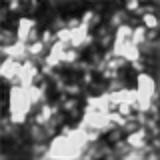
\includegraphics[scale=0.32]{/home/dimitrios/_Publication_Latex/_Big_Data_From_Space_2017/Images/generated_data_80x80_upsampled/126000_00708.jpg}  & 
			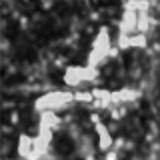
\includegraphics[scale=0.32]{/home/dimitrios/_Publication_Latex/_Big_Data_From_Space_2017/Images/generated_data_80x80_upsampled/126000_00734.jpg}  & 
			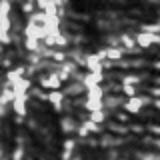
\includegraphics[scale=0.32]{/home/dimitrios/_Publication_Latex/_Big_Data_From_Space_2017/Images/generated_data_80x80_upsampled/129000_00130.jpg}  & 
			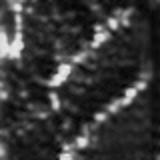
\includegraphics[scale=0.32]{/home/dimitrios/_Publication_Latex/_Big_Data_From_Space_2017/Images/generated_data_80x80_upsampled/129000_00141.jpg}  & 
			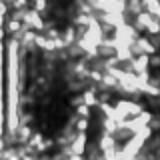
\includegraphics[scale=0.32]{/home/dimitrios/_Publication_Latex/_Big_Data_From_Space_2017/Images/generated_data_80x80_upsampled/168000_00706.jpg}  &
   			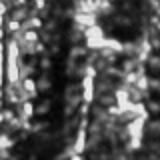
\includegraphics[scale=0.32]{/home/dimitrios/_Publication_Latex/_Big_Data_From_Space_2017/Images/generated_data_80x80_upsampled/168000_00773.jpg}  &
   			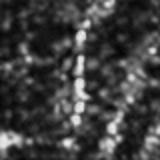
\includegraphics[scale=0.32]{/home/dimitrios/_Publication_Latex/_Big_Data_From_Space_2017/Images/generated_data_80x80_upsampled/168000_00806.jpg}  \\
   			
   			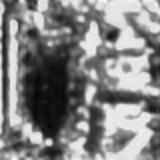
\includegraphics[scale=0.32]{/home/dimitrios/_Publication_Latex/_Big_Data_From_Space_2017/Images/generated_data_80x80_upsampled/168000_00832.jpg}  &
   			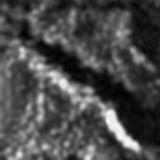
\includegraphics[scale=0.32]{/home/dimitrios/_Publication_Latex/_Big_Data_From_Space_2017/Images/generated_data_80x80_upsampled/186000_00700.jpg}  &   			
   			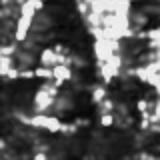
\includegraphics[scale=0.32]{/home/dimitrios/_Publication_Latex/_Big_Data_From_Space_2017/Images/generated_data_80x80_upsampled/186000_00704.jpg}  & 
   			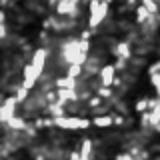
\includegraphics[scale=0.32]{/home/dimitrios/_Publication_Latex/_Big_Data_From_Space_2017/Images/generated_data_80x80_upsampled/186000_00707.jpg}  & 
   			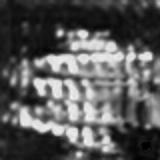
\includegraphics[scale=0.32]{/home/dimitrios/_Publication_Latex/_Big_Data_From_Space_2017/Images/generated_data_80x80_upsampled/186000_00720.jpg}  &
   			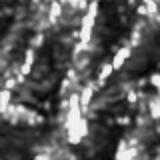
\includegraphics[scale=0.32]{/home/dimitrios/_Publication_Latex/_Big_Data_From_Space_2017/Images/generated_data_80x80_upsampled/186000_00760.jpg}  &
   			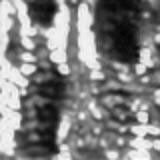
\includegraphics[scale=0.32]{/home/dimitrios/_Publication_Latex/_Big_Data_From_Space_2017/Images/generated_data_80x80_upsampled/129000_00150.jpg}  \\
   			
	\multicolumn{7}{c}{\textbf{Figure 1.} Generated data of size $80 \times 80$ pixel by cropping scenario - upsampled to $160 \times 160$ pixel}
	\end{tabular}
	\label{generated-data}
\end{table*}

\begin{table*}[t]
	\centering
	\begin{tabular}{ccccccc}
			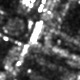
\includegraphics[scale=0.64]{/home/dimitrios/_Publication_Latex/_Big_Data_From_Space_2017/Images/real_image_samples/1.png}  & 
			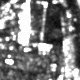
\includegraphics[scale=0.64]{/home/dimitrios/_Publication_Latex/_Big_Data_From_Space_2017/Images/real_image_samples/2.png}  & 
			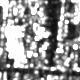
\includegraphics[scale=0.64]{/home/dimitrios/_Publication_Latex/_Big_Data_From_Space_2017/Images/real_image_samples/3.png}  & 
			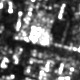
\includegraphics[scale=0.64]{/home/dimitrios/_Publication_Latex/_Big_Data_From_Space_2017/Images/real_image_samples/4.png}  & 
			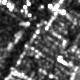
\includegraphics[scale=0.64]{/home/dimitrios/_Publication_Latex/_Big_Data_From_Space_2017/Images/real_image_samples/5.png}  &
   			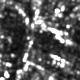
\includegraphics[scale=0.64]{/home/dimitrios/_Publication_Latex/_Big_Data_From_Space_2017/Images/real_image_samples/6.png}  &
   			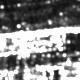
\includegraphics[scale=0.64]{/home/dimitrios/_Publication_Latex/_Big_Data_From_Space_2017/Images/real_image_samples/7.png}  \\
   			
   			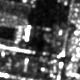
\includegraphics[scale=0.64]{/home/dimitrios/_Publication_Latex/_Big_Data_From_Space_2017/Images/real_image_samples/8.png}  &
   			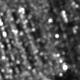
\includegraphics[scale=0.64]{/home/dimitrios/_Publication_Latex/_Big_Data_From_Space_2017/Images/real_image_samples/9.png}  &   			
   			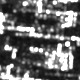
\includegraphics[scale=0.64]{/home/dimitrios/_Publication_Latex/_Big_Data_From_Space_2017/Images/real_image_samples/10.png}  & 
   			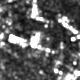
\includegraphics[scale=0.64]{/home/dimitrios/_Publication_Latex/_Big_Data_From_Space_2017/Images/real_image_samples/11.png}  & 
   			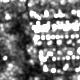
\includegraphics[scale=0.64]{/home/dimitrios/_Publication_Latex/_Big_Data_From_Space_2017/Images/real_image_samples/12.png}  &
   			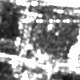
\includegraphics[scale=0.64]{/home/dimitrios/_Publication_Latex/_Big_Data_From_Space_2017/Images/real_image_samples/13.png}  &
   			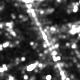
\includegraphics[scale=0.64]{/home/dimitrios/_Publication_Latex/_Big_Data_From_Space_2017/Images/real_image_samples/14.png}  \\
   			
	\multicolumn{7}{c}{\textbf{Figure 2.} Original \emph{TerraSAR-X} data of original size - $160 \times 160$ pixel}
	\end{tabular}
	\label{real-data}
\end{table*}


% To start a new column (but not a new page) and help balance the last-page
% column length use \vfill\pagebreak.
% -------------------------------------------------------------------------
%\vfill
%\pagebreak

%\section{REFERENCES}
%\label{sec:ref}


% References should be produced using the bibtex program from suitable
% BiBTeX files (here: strings, refs, manuals). The IEEEbib.bst bibliography
% style file from IEEE produces unsorted bibliography list.
% -------------------------------------------------------------------------
\bibliographystyle{IEEEbib}
\bibliography{strings,refs}

\end{document}
